% Principal GDZ PPN236018647, native466–467; HKUST467–468.
\clearpage\SourceLeaf{466}\NoSourceHead
\pdfbookmark[1]{Geometrie: Briefwechsel}{geometry-correspondence}
\HistoricTitle{\textls[180]{BRIEFWECHSEL.}}
\NumberedItem{1}
\begin{center}\textsc{Schumacher} an \textsc{Gauss}.\quad Altona, 19. März 1836.\end{center}
\HistoricCitation{[Briefwechsel zwischen \textsc{Gauss} und \textsc{Schumacher} III, Altona 1861, S. 7—8.]}
\indent \{.\enspace.\enspace.\enspace.\quad Mir ist neulich ein Paradox vorgekommen, das ich so frei bin Ihnen vorzulegen. Ich kann es noch nicht genügend erklären.

\indent Bekanntlich ist, wenn man bei einem Vierecke \(ABCD\) einen Punct sucht, von dem die Summe der an die Winkelpuncte gezogenen Linien ein Minimum sey, der gesuchte Punct der Durchschnittspunct der Diagonalen \(E\). Lässt man nun die Puncte \(A,\ B\) in den Linien \(DA,\ BC\) immer mehr hinaufrücken, bis sie am Ende in \(F\) zusammenfallen, so fällt auch \(E\) zugleich in \(F\), das Viereck verwandelt sich in das Dreieck \(DFC\), und man hätte den Punct \(F\) als denjenigen, von dem die Summe der an die Winkelpuncte \(F,\ C,\ D\) des Dreiecks gezogenen Linien ein Minimum sey. Das ist aber bekanntlich nur wahr, wenn der Winkel \(F\geqq120^{0}\).
\begin{center}
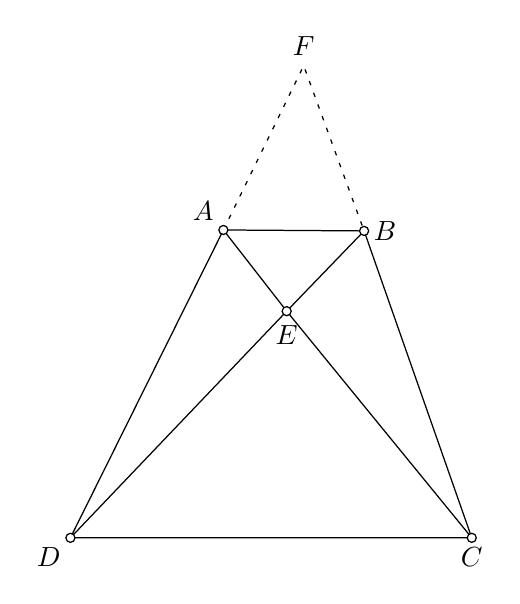
\begin{tikzpicture}[x=.012cm,y=-.012cm,line width=.45pt]
\draw (0,500)--(162,174)--(311,175)--(425,500)--cycle;
\draw (162,174)--(229,260)--(425,500);
\draw (0,500)--(229,260)--(311,175);
\draw[dash pattern=on 1.6pt off 2.9pt] (162,174)--(247,0)--(311,175);
\draw[fill=white] (0,500) circle[radius=4.8];
\draw[fill=white] (425,500) circle[radius=4.8];
\draw[fill=white] (162,174) circle[radius=4.8];
\draw[fill=white] (311,175) circle[radius=4.8];
\draw[fill=white] (229,260) circle[radius=4.8];
\node[above left] at (162,174) {$A$};
\node[right] at (311,175) {$B$};
\node[below] at (425,500) {$C$};
\node[below left] at (0,500) {$D$};
\node[below] at (229,265) {$E$};
\node[above] at (247,0) {$F$};
\end{tikzpicture}
\end{center}

\indent Noch mehr; man kann dieselbe Construction bei jedem der andern beiden Winkelpuncte des Dreiecks machen, und würde, wenn die Seiten des Dreiecks \(a,\ b,\ c\) sind, so 3 Gleichungen erhalten:
\par\vfill\noindent\hfill 58\textsuperscript{*}
\clearpage\SourceLeaf{467}\ArithmeticHead{460}{L}{GEOMETRIE. BRIEFWECHSEL.}
\[
\begin{aligned}
a+b&=\text{Minimum}\\
b+c&=\text{Minimum}\\
a+c&=\text{Minimum},
\end{aligned}
\]
\noindent also \(a+b=b+c=a+c\), welches absurd ist. Es folgt daraus \(a=b=c\).

\indent Ebenso wenn man das Viereck \(ABCD\) betrachtet, so ist der gesuchte Punct wiederum \(E\). Lässt man nun \(D\) auf \(AD\) immer gegen \(E\) rücken, bis dieser Punct in \(CB\) fällt, so verwandelt sich das Viereck in das Dreieck \(ABC\) und der gesuchte Punct muss, da der Schnitt aufhört, irgendwo in der Linie \(CB\) liegen. Offenbar erfüllt jeder Punct in dieser Linie (der zwischen \(C\) und \(B\) liegt\footnotemark{}) die Bedingung für die Puncte \(C,\ B\); soll er sie auch für den Punct \(A\) erfüllen, so muss es das Perpendikel von \(A\) auf \(CB\) seyn. Ebenso kann man bei jeder der andern beiden Seiten des Dreiecks raisonniren. Wenn also die Seiten \(s,\ s',\ s''\), die darauf gefällten Perpendikel \(p,\ p',\ p''\) sind, so hat man:
\footnotetext{auch \(C\) und \(B\) selbst. Dann ist
\[\begin{aligned}BC+BA&=\text{Minimum}\\CA+BC&=\text{Minimum},\end{aligned}\]
\noindent also \(CA=BA\), quod absurdum.}
\begin{center}
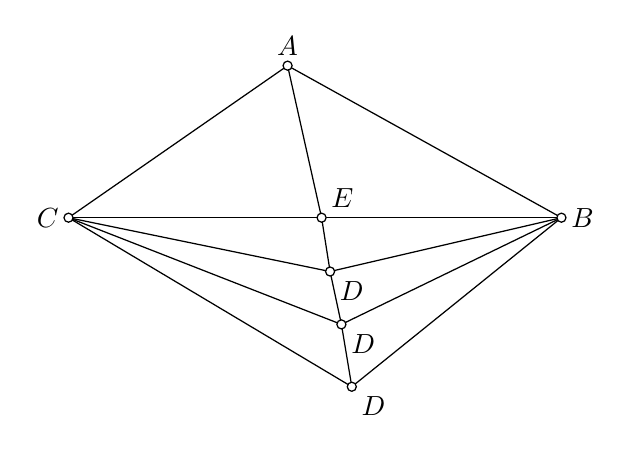
\begin{tikzpicture}[x=.012cm,y=-.012cm,line width=.45pt]
\draw (0,161)--(232,0)--(522,161)--(300,340)--cycle;
\draw (0,161)--(268,161)--(522,161);
\draw (232,0)--(268,161)--(277,218)--(289,274)--(300,340);
\draw (0,161)--(277,218)--(522,161);
\draw (0,161)--(289,274)--(522,161);
\draw[fill=white] (0,161) circle[radius=4.8];
\draw[fill=white] (232,0) circle[radius=4.8];
\draw[fill=white] (522,161) circle[radius=4.8];
\draw[fill=white] (268,161) circle[radius=4.8];
\draw[fill=white] (277,218) circle[radius=4.8];
\draw[fill=white] (289,274) circle[radius=4.8];
\draw[fill=white] (300,340) circle[radius=4.8];
\node[above] at (232,0) {$A$};
\node[right] at (522,161) {$B$};
\node[left] at (0,161) {$C$};
\node[above right] at (268,161) {$E$};
\node[below right] at (277,218) {$D$};
\node[below right] at (289,274) {$D$};
\node[below right] at (300,340) {$D$};
\end{tikzpicture}
\end{center}
\[
\begin{aligned}
s+p&=\text{Min.}\\
s'+p'&=\text{Min.}\\
s''+p''&=\text{Min.},
\end{aligned}
\]
\noindent also \(s+p=s'+p'=s''+p''\), welches wiederum absurd ist, da bekanntlich:
\[sp=s'p'=s''p''.\text{\}}\]
